\chapter{Introduction}
\chaptermark{Introduction}
\label{ch:introduction}


	

Square-law detection, also known as Direct detection (DD), is a detection scheme that measures the square magnitude of a complex wave form, clearly this scheme is a nonlinear waveform detection because of the square operation. Direct detection is widely used in different scientific fields, for example in crystallography, radio astronomy, biomedical spectroscopy, among others \cite{Tasbihi_Tukey}. In particular this scheme is often used in optical communications, specially in short-haul systems with length up to \SI{50}{\km} \cite{Agrawal_ch1} due to its simplicity, or even in shorter links up to \SI{10}{\km} for example in rack to rack communications in big data centers.\\
\nomenclature{DD}{Direct Detection}

In the recent years the interest of studying systems with DD is getting bigger again, because of the simplicity of the receivers, which are a promising low-cost alternative compared to the coherent detection systems \cite{Mecozzi_2018}. In this context two questions or problems arise. First, how good is a system with DD compared to a system with coherent detection in terms of the information capacity of the channels. And second, how to design a system that exploits the information capacity of the DD channel in the best possible way.\\

In this work we cover briefly two answers given to the first question, and then we review two systems proposed for a channel with DD. Then we propose a new decoder for the second system, with reduced complexity at the expenses of a slightly worse performance.




\section{Direct Detection}
\label{sec:Direct_Detection}

In optical communication DD is performed with a single photodiode, that convert the optical signal to an electric signal trough the photoelectric effect according to the next equation \cite{Agrawal_ch4}:
\begin{equation}
I_p = R_d\cdot P_{in}
\label{eq:photocurrent}
\end{equation}
where $I_p$ is the photocurrent, $P_{in}$ is the incident optical power (which is proportional to the square of the magnitud of the electric field, that is where the square-law term comes from), and $R_d$ is the so called responsivity of the photodetector, with units of \SI{}{\A/\W}.\\

The noise in the photodiode are generated primarily by two mechanisms, in the first place the shot noise, and in the second place thermal noise.\\

The shot noise is models the fact that the photocurrent consist of a stream of electrons generated at random times. Mathematically the current corresponding to the shot noise $i_s(t)$ is a stationary random process with Poisson distribution, but is usually approximated by a Gaussian distribution with variance given by \cite{Agrawal_ch4}:
\begin{equation}
\sigma_s^2 = 2qI_pB
\label{eq:shot_noise_varaince}
\end{equation}
where $q$ is the electron charge, $I_p$ the photocurrent, and $B$ the bandwidth of the system. $\sigma_s$ can be interpreted as the RMS value of the shot noise current $i_s(t)$.\\ 

The termal noise is generated by the movement  of electrons due to the ambient temperature, and the variance of the noise is given by \cite{Agrawal_ch4}:
\begin{equation}
\sigma_{th}^2 = \frac{4k_BT}{R_L} F_nB
\label{eq:thermal_noise_variance}
\end{equation}
where $k_B$ is the Boltzmann constant, $T$ is the temperature given in kelvin, $R_L$ is the load resistance, $B$ the bandwidth, and $F_n$ is the amplifier noise figure. \\

With this in mind the output current of the direct detection process is given by:
\begin{equation}
I(t) = I_p+i_s(t)+i_{th}(t)
\label{eq:DD_current}
\end{equation}
with $i_s(t)\sim\mathcal{N}(0,\sigma_s^2)$ and $i_{th}(t)\sim\mathcal{N}(0,\sigma_{th}^2)$
\nomenclature{$X\sim\mathcal{N}(\mu,\sigma^2)$}{$X$ has a Gaussian distribution with mean $\mu$ and variance $\sigma^2$}


\section{Capacity under direct detection}
\label{sec:capacity_under_direct_detection}

A communications channel that uses DD can retrieve only the information about the magnitude of the signal, in contrast a system with coherent detection can retrieve the magnitud and phase of the signal. This means that DD scheme ignores one of the two degrees of freedom, and hence it is reasonable to think that the capacity of this systems should be approximately half that of the system with coherent detection \cite{Mecozzi_2018, Tasbihi_Tukey, Tasbihi_Capacity}.\\

However in \cite{Mecozzi_2018} it is shown that the spectra efficiency of a band limited system under DD is at most \SI{1}{bit/\s/\Hz} less than the same system under coherent detection. Also in \cite{Tasbihi_Capacity} it is proven that for time limited signals  the capacity is also at most one bit les than the coherent case. This means that contrary to intuition, the loss in the capacity of a system under DD is not a half of the coherent system, but just \SI{1}{bit/\s/\Hz}.\\

The results of this papers show that the systems with DD have a big potential, because the detector are cheaper and easier to implement (basically just one photodiode) and the loss in the capacity may not be as big as thought. However the problem to find a system simple enough that uses the potential of the DD is still open. 



\section{Basic principle of phase recovery}

The key to retrieve the phase information of the transmitted symbols when using DD is to make use of the ISI. As a toy example one can think on the problem where given two complex numbers $z_1$ and $z_2$, from $|z_1|^2$, $|z_2|^2$ and $|z_1+z_2|^2$ (an ISI term), it is possible to determine the phase difference between $z_1$ and $z_2$ up to a sign ambiguity \cite{Tasbihi_Tukey}.\\

To show this, notice the following:
\begin{align*}
	|z_1+z_2|^2 &= (z_1+z_2)(z_1+z_2)^* \\
	&=z_1z_1^*+z_1z_2^*+z_2z_2^*+z_1^*z_2\\
	&=|z_1|^2+|z_2|^2+z_1z_2^*+\bigl(z_1z_2^*\bigr)^*\\
	&=|z_1|^2+|z_2|^2+2\text{Re}\{z_1z_2^*\}\\
\end{align*}
under the convention that $z_1 = a\cdot e^{j\alpha}$ and $z_2 = b\cdot e^{j\beta}$
\begin{equation}
	|z_1+z_2|^2 =|z_1|^2+|z_2|^2+2|z_1||z_2|\cos(\alpha-\beta)\\
	\label{eq:square_mag_of_sum}
\end{equation}
\nomenclature{$j$}{Imaginary unit}
\nomenclature{Re$\{z\}$}{Real part of $z$}
\nomenclature{Im$\{z\}$}{imaginary part of $z$}

Clearly if $|z_1|^2$, $|z_2|^2$ and $|z_1+z_2|^2$ are known, one can solve the equation \ref{eq:square_mag_of_sum} for $\cos(\alpha-\beta)$ and get the information about the phase difference between $z_1$ and $z_2$. However, since cosine is an even function $\cos(\alpha-\beta)=\cos(-\alpha+\beta)$, hence there is still an ambiguity on the sign of the phase difference.\\


\begin{figure}[htb]
     \centering
     \begin{subfigure}[b]{0.49\textwidth}
         \centering
         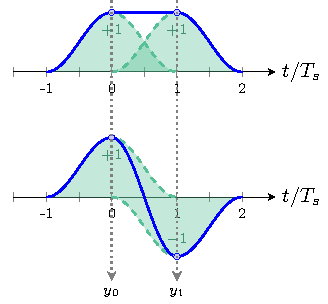
\includegraphics[width=\textwidth]{images/CD_toy_example.pdf}
         \caption{Coherent detection}
         \label{fig:CD_toy_example}
     \end{subfigure}
     \hfill
     \begin{subfigure}[b]{0.49\textwidth}
         \centering
         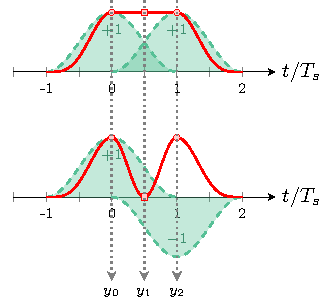
\includegraphics[width=\textwidth]{images/DD_toy_example.pdf}
         \caption{Direct detection}
         \label{fig:DD_toy_example}
     \end{subfigure}
     \hfill
     \vspace{10mm}
     \begin{subfigure}[b]{0.8\textwidth}
         \centering
         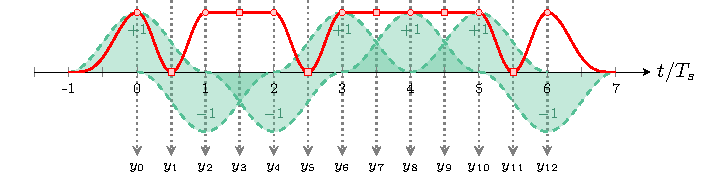
\includegraphics[width=\textwidth]{images/DD_toy_example_long_sq.pdf}
         \caption{Direct detection of the sequence $\{+1,-1,-1,+1,+1,+1,-1\}$}
         \label{fig:DD_toy_example_long_sq}
     \end{subfigure}
        \caption{Comparative of the wave forms under coherent detection and direct detection. Based on \cite{Secondini, Plabst_DD}.}
        \label{fig:DD_vs_CD}
\end{figure}

To visualize this principle in a real system (jet not even near to optimal due to the big bandwidth of the pulse), see the figure \ref{fig:DD_vs_CD}. There is shown with a solid line the wave form of a simple transmission under coherent detection (see figure \ref{fig:CD_toy_example}) and under direct detection (see figure \ref{fig:DD_toy_example}), and also the wave form of the individual symbols in dashed lines.\\

For the coherent detection case the samples at each symbol time are sufficient to determine the transmitted symbols. In contrast, for the direct detection case the samples at each symbol time (circles) only carry information about the magnitude of the symbols (always one in this example); and the samples at intermediate symbol time (squares) carry information about the phase difference \cite{Secondini}.\\

Figure \ref{fig:DD_toy_example_long_sq} show the DD system for a longer sequence, there it is possible to notice that the even samples always carry information about the magnitude, whereas the odd samples carry information about the differential phase of the symbols. This toy example shows the principle behind the phase recovery in DD systems, it is important to highlight two things, first an oversampling factor of two is needed, and second only information on the differential phase (up to a sign ambiguity) is retrieved, hence it is beneficial to use differential coding in the transmission.\\

An other way to explain the previous conclusions is to take a look at the simple system given by:
\begin{align*}
	g(t)=\sum_{k=0}^m g_k\text{sinc}(t-k)
\end{align*}
where $g_k$ is a complex number representing the transmitted symbol and $g(t)$ is the transmitted signal. Note that after the DD the bandwidth of the signal is twice as big as the bandwidth of $g(t)$, since the received signal is given by the product $|g(t)|^2=g(t)g^*(t)$. Hence to recover the data one should use an oversampling factor of two, so the sampled signal becomes \cite{Tasbihi_Tukey}:
\begin{align*}
	\left|g\left(\frac{n}{2}\right)\right|^2 = \left\{
\begin{array}{ll}
\left|g_{\frac{n}{2}}\right|^2  &  \text{if $n$ is even}  \\
\left|\sum\limits_{k=0}^m g_k\text{sinc}\left(\frac{n}{2}-k\right)\right|^2   & \text{if $n$ is odd}
\end{array}
\right. &&\text{for }n=0,\dotsb,2m
\end{align*}
\nomenclature{sinc$(t)$}{$\frac{\sin(\pi t)}{\pi t}$}

Once again, it is clear that the even samples carry the information about the magnitude of the symbols, whereas the odd samples carry some how the information about the phase of the symbols. But now notice that all the $g_k$ contribute to the odd samples, this makes that retrieving the phase becomes quickly an intractable problem as $m$ grows \cite{Tasbihi_Tukey}, as we will see in later chapters. 

















